
\chapter{Edit selected surfaces}
\minitoc 
As a prerequisite, you need to select surfaces. Only selected surfaces can be edited. 
\section{Structure modifications}
\subsection{Invert}
\noindent
\begin{minipage}{0.3\textwidth}

A given surface's triangles can be
inverted in order to show inner structures.\\

Note that the original surface
is directly affected; this option
does not involve the use of a
filter (no output additional
surface is created).
\end{minipage}  
 \begin{minipage}{0.6\textwidth}\centering
  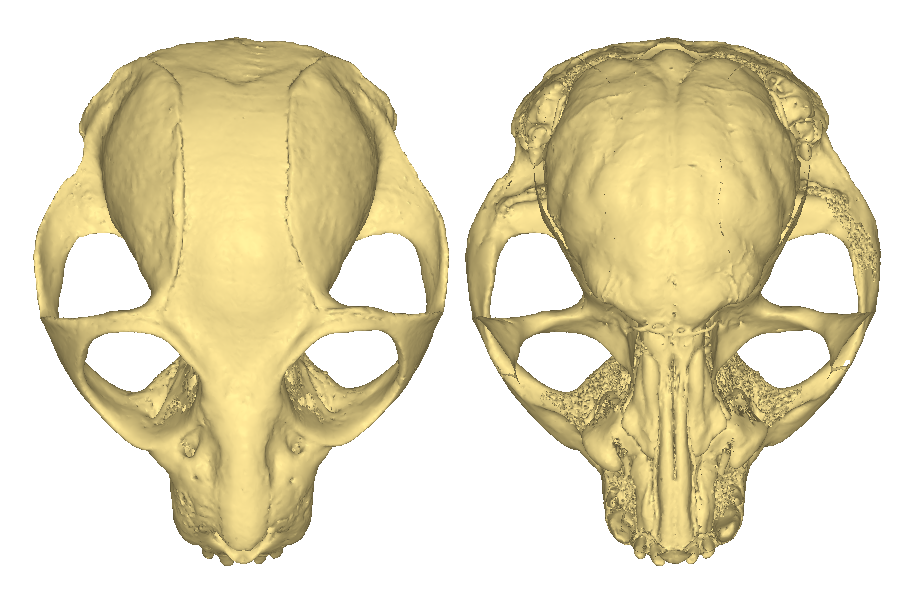
\includegraphics[scale=0.35]{images/Edit_selected_objects/01_invert.png}
 \captionof{figure}{Example of surface triangle inversion. Left: original surface.
Right: the same surface inverted, revealing inner structures such
as the endocranial cavity. Gouraud shading rendering + backface
culling option was used.}
 \end{minipage} 
\noindent




\subsection{Mirror}

This option uses vtkReflectionFilter,which produces a mirror image of the original selected input mesh.\\

\begin{figure}
  \centering
  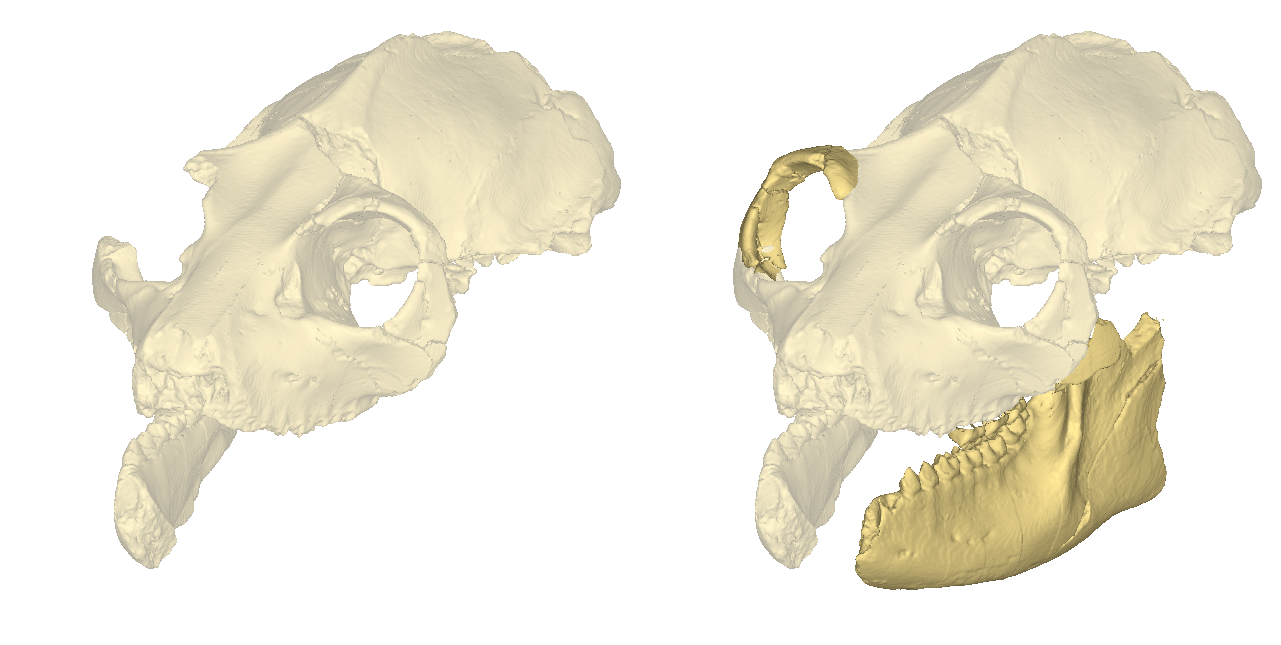
\includegraphics[scale=0.35]{images/Edit_selected_objects/02_Mirror.png} 
	\caption{Example of fossil restoration implicating the production of mirror images of missing parts.}
 
\end{figure}

\subsection{Connectivity : separate all non connected regions}

Connectivity decomposition window\\

Original surface containing a large number of independent regions of size > 350 triangles (in grey)\\

Filtered surfaces : all meshes produced using this filter have more than 350 triangles\\

Left: original surface (one single mesh). Right: the resulting 298 filter output surfaces (each drawn using a different colour) can be manipulated independently.\\


This option uses vtkPolyDataConnectivityFilter. This filter produces a new surface for each non-connected region of the selected input surface. 3D meshes of biological objects sometimes contain a multitude of small and biologically irrelevant independent regions. This ``noise" may have multiple origins: low quality of original 3D data, state of preservation of the specimen, threshold used to be able to visualize all relevant structures, etc... In order to extract relevant independent regions, only regions reaching a minimal size (minimal number of triangles) are transformed into new surfaces. This process may take some time to be completed. All produced surfaces corresponding to independent regions can be manipulated independently.



\subsection{Connectivity: keep largest region}
This option uses vtkPolyDataConnectivityFilter.This filter produces a new surface for the largest independent region of the selected input surface.\\

Left: original surface. Right: the resulting largest region in terms of triangle number.

\subsection{Lasso cut}
You may cut through an input selected surface using this option. Once ``lasso cut" menu is clicked, the mouse cursor changes to a cross in the 3D window. Additional mouse and keyboard controls become available.\\
\rowcolors{2}{}{gray!25}

\begin{tabularx}{\linewidth}{ | c | X | }
\hline			
Left click & Adds a segment to polygon (segments are drawn yellow) \\ \hline			

Right click & Connects last segment to first segment. If two segments cross each other, lasso action is cancelled. Otherwise, the closed polygon is drawn red.\\ \hline			

Middle click or ``C" + right click. & Once the lasso is closed (lasso polygon drawn red
after a right click):\newline
when click falls inside/outside the closed red polygon: the region falling inside the polygon is included/is not included into the filter output surface, respectively. The region falling ousitde the polygon is not included/is included inside the output, respectively.

\\ \hline	
			
	
\end{tabularx}

Once ``Middle click" is pressed or ``C" + right click is pressed, the usual mouse and keyboard controls become available again.\\

Left clicks $\rightarrow$ add new yellow segments\\

Right final click $\rightarrow$ connects last segment to first segment\\

Result of middle click inside red polygon.\\

Left clicks $\rightarrow$ add new yellow segments\\
Right final click $\rightarrow$ connects last segment to first segment \\

Result of middle click outside red polygon.\\

\subsection{Smooth}
Smoothing window\\

Left: example of original input surface. Right: resulting output surface after 50 iterations using a relaxation factor of 0.1.\\

This option uses vtkSmoothPolyDataFilter.You may smooth an input
selected surface using this option. A number of iteration and a
relaxation factor are required.\\
See vtkSmoothPolyDataFilter documentation for further information regarding this option.

\subsection{TPS deformation}
TPS window\\
Original distorted input surface. 31 ``normal"
landmarks were placed on the surface and 31
``target" landmarks were placed in order to
restore bilateral symmetry.\\
Resulting output (deformation : 100\%). Note
that the 31 ``target" landmarks are located on
the output surface.




This option uses vtkThinPlateSplineTransform filter.
Requirements : to use TPS deformation, a selected surface,
a series of ``n" normal landmarks and a series of ``n"
target landmarks (n>3) are needed. ``Normal" landmarks
are usually placed on the original selected input surface,
whereas ``target" landmarks are placed at a location in 3D
space which will drive the TPS deformation. See vtkThinPlateSplineTransform documentation for further information regarding TPS deformation.

\subsection{Decimate}
Decimate window\\
This option uses vtkDecimatePro and
vtkQuadricDecimation filters.
Requirements : to use mesh decimation, a selected
surfaceis required.
See vtkDecimatePro and vtkQuadricDecimation documentations for further information regarding
mesh decimation.\\

Original input surface. Number of triangles: 27679.\\
Resulting output (vtkQuadricDecimation filter,
decimation factor: 80\%). Number of triangles:5535.

\subsection{Densify}
Densify window\\
Original input surface. Number of triangles: 5535.\\

Resulting output (number of subdivisions: 1). Number of triangles: 16605.\\


This option uses vtkDensifyPolyData filter.
Requirements : to use mesh densification, a selected
surfaceis required.
Note that mesh decimation can become extremely slow
when using number of subdivisions larger than 1.
See vtkDensifyPolyData documentation for further information regarding mesh densification.

\subsection{Fill holes}
Fill holes window\\
Original input surface. Number of triangles: 5535. \\
Resulting output (maximal size: 1). Number of triangles: 5689.\\


This option uses vtkFillHolesFilter.
Requirements : to use mesh hole filling, a selected surfaceis
required. See vtkFillHolesFilter documentation for further
information regarding hole filling.


\section{Rendering modifications.}
\subsection{Set alpha value}
A selected surface is needed.\\
Please chose a value between 0 and 100. 100 stands for ``opaque
rendering". 0 stands for ``invisible surface".\\
As stated earlier, vertex display order has consequences on 3D rendering when working with
transparency. 3D objects are displayed one after the other following an object list. The way object are ordered inside this list thus affects transparency rendering, especially when some objects such as inner structures are positioned inside others. Object display order of selected objects can be changed using the two following controls. Pressing ``
\includegraphics[scale=0.7]{images/pixmap/s_dessous_17.png}" will place all selected objects one step earlier in the object display list. Pressing ``
\includegraphics[scale=0.7]{images/pixmap/s_dessus_17.png}" will place all selected objects one step further in the object display
list.\\

See also ``Sort vertices from back to front (beware: slow rendering)" and ``Sort vertices from front to back (beware: slow rendering)" sections for further information.\\


1) 3 objects (cranium, left\_inner\_ear and right\_
inner\_ear) are opened in this order, and object
``cranium" is rendered with an alpha value of 40.
The inner ears remain invisible, because ``cranium"
is displayed before the two inner ears\\
Corresponding display object order (Show $\rightarrow$Display
object order)\\
2) ``Cranium" was selected, and button ``
\includegraphics[scale=0.7]{images/pixmap/s_dessus_17.png}" was
pressed. Now the left inner ear is visible, because
it is displayed before the cranium.\\
Corresponding display object order\\

3) ``Cranium" was selected again, and button ``
\includegraphics[scale=0.7]{images/pixmap/s_dessus_17.png}" was pressed. Now the two inner ears are
visible, because they are displayed before the
cranium.\\
Corresponding display object order


\subsection{Change object colour}
Object colour can be changed using this option. A set of 13 predefined colours is available via this menu. Alternatively, you can edit object colour manually using the ``Object colour" control of the ``General options" window (click on menu ``Show $\rightarrow$General options$\rightarrow$").

\subsection{Edit first selected object and aspect matrices}
Object matrix window\\

A selected surface is required . This opens the following window,
in which the aspect and position matrices can be edited.
Options :\\
- Ok : set aspect and position matrices to first selected object.\\
- Init : set aspect and position matrices to identity.\\
- Refresh : change matrices to those of first selected object.\\
- Ok for all selected objects: set aspect and position matrices to
all selected objects.\\
You can also access faster the ``Object Matrix" window by clicking
on ``
\includegraphics[scale=0.7]{images/pixmap/mat.png}"(edit first selected object position and aspect matrices).

\section{Grouping actions.}
One or several meshes can be placed into one logical object using this option. This option is useful in the following two cases.\\
- It allows an easy way to select/unselect together several objects (sometimes you do not want
to select/unselect manually multiple meshes one by one).\\
- As a logical object’s aspect object and position matrices can be edited, placing 1 or several
meshes into one logical object provides a convenient means to achieve deformation into
a particular direction in 3D space (for instance to achieve mesh decompression in one
direction.\\
Logical objects can be also put into another logical object. Note that meshes contained into selected logical objects cannot be saved until they are ungrouped.

\subsection{Group}
Select one or several meshes. Click on ``Edit selected surfaces$\rightarrow$Grouping actions$\rightarrow$Group". As a result, the selected meshes are drawn in brown colour.
\subsection{Ungroup}
Select one logical object. Click on ``Edit selected surfaces$\rightarrow$Grouping actions$\rightarrow$Ungroup". If the logical object aspect and position matrices are different from the identity matrices, the position and aspect matrices of the contained objects are edited in order to take into account position and aspect transformations that were applied to that logical object. Then the objects contained into the selected logical object are ungrouped, and the selected logical object is deleted.\\

1) 7 objects are opened. Original matrices of ``bx\_md" object are shown (right mandible, selected).\\
Corresponding display object order (Show $\rightarrow$Display object order)\\
2) The 7 object are grouped. The group is drawn in brown. \\
Corresponding display object order\\

3) The position of the group is changed, as well as its aspect matrix. Note that the enclosed meshes cannot be saved in that state.\\
Corresponding display object order\\

4) Objects are ungrouped. Modified matrices of ``bx\_md" object are shown (right mandible is selected). Now, the 7 meshes can be saved.\\
Corresponding display object order (Show $\rightarrow$Display object order)

\section{Object list order..}
As explained earlier, the following options are useful when working with transparent objects. Normal and Target landmark ordering can also be edited using these options.
\\As stated above, access to object display order can be reached via the menu ``Show$\rightarrow$Display object order".

\subsection{Move up}
All selected objects (landmarks or surfaces) will be placed one step earlier in the object display list.
This action can also be reached via the following button:
\includegraphics[scale=0.7]{images/pixmap/s_dessous_17.png}

\subsection{Move down}
All selected objects (landmarks or surfaces) will be placed one step further in the object display list.
This action can also be reached via the following button:
\includegraphics[scale=0.7]{images/pixmap/s_dessus_17.png}
See tutorial ``working with landmarks" for further information.

\section{Delete small objects.}
\subsection{Threshold : a given number of triangles}
Delete small objects window\\

Using this option, you may delete selected objects smaller than a given number of triangles.

\subsection{Threshold : a given volume}
Delete small objects window 2\\
Using this option, you may delete selected objects smaller than
a given volume.
